\documentclass[preview,convert={density=800,outext=.png}]{standalone}
%\documentclass[preview]{standalone}

\usepackage[utf8]{inputenc}				% Кодировка utf8

\usepackage{tikz}
\usetikzlibrary{calc,patterns,backgrounds,arrows}

\newcommand{\blockp}[3]{
	\node[draw, rectangle, pattern = #3, minimum width = #1, minimum height = #2, preaction={fill, white}] 
}
\begin{document}
	
	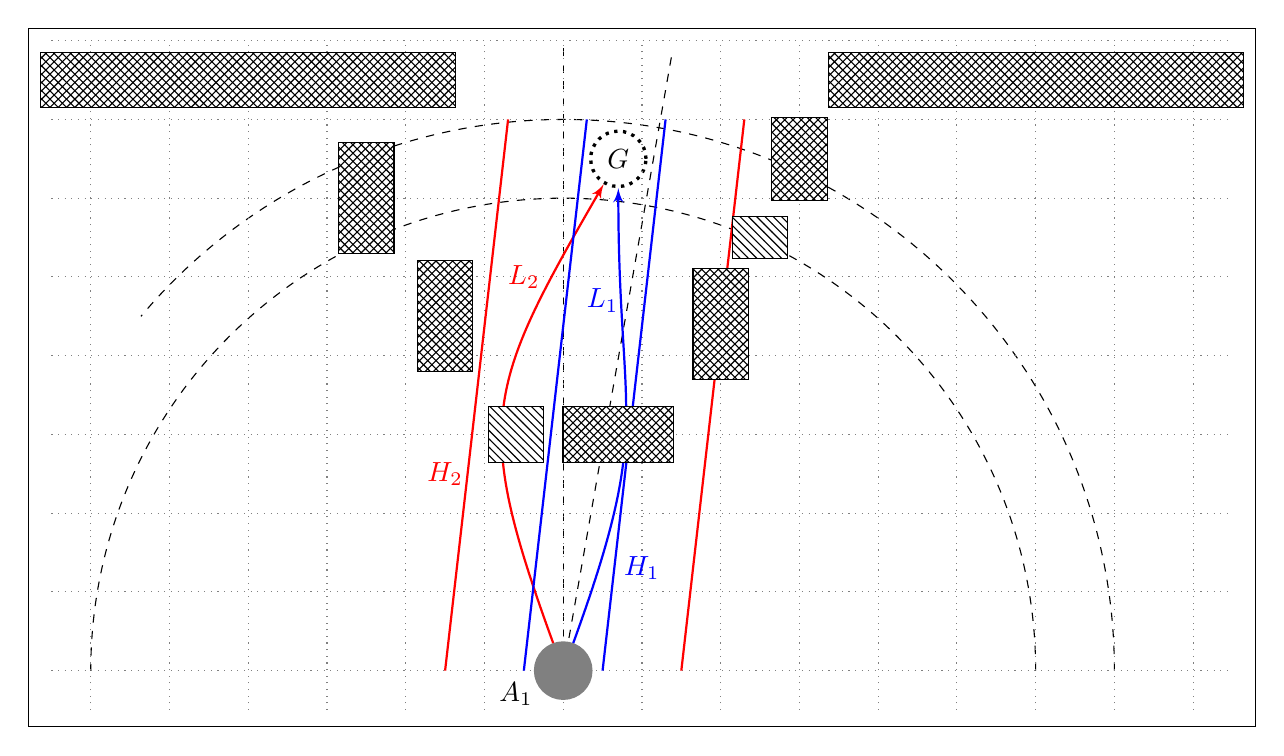
\begin{tikzpicture}[framed]
		\draw[dashed] (4,-7.5) ++(0:6) arc (0:180:6);
		\draw[dashed] (4,-7.5) ++(0:7) arc (0:140:7);
		\draw[dashed] (4,-7.5) -- ++(90:8);
		\draw[dashed] (4,-7.5) -- ++(80:8);

		\node[draw, circle, dotted, very thick, minimum width = 20, text = black] (goal) at (4.7, -1) {$G$};
				
		\node[draw, gray, fill = gray, circle, very thick, minimum width = 20] (obj_1) at (4, -7.5) {};
		
		\draw[step=1,gray,dotted, yshift=-0.5cm] (-2.5,-7.5) grid (12.5,1);
		\draw [-latex', blue, thick] (obj_1) to[out=70,in=-90, distance=3cm ] (goal);
		\draw [-latex', red, thick] (obj_1) to[out=110,in=-120, distance=3cm ] (goal);
		
		\node at (3.4, -7.8) {$A_1$};
		\node[red] at (2.5, -5) {$H_2$};
		\node[red] at (3.5, -2.5) {$L_2$};
		\node[blue] at (5, -6.2) {$H_1$};
		\node[blue] at (4.5, -2.8) {$L_1$};
				
		\draw[blue, thick] (3.5,-7.5) -- (4.3, -0.5);
		\draw[blue, thick] (4.5,-7.5) -- (5.3, -0.5);

		\draw[red, thick] (2.5,-7.5) -- (3.3, -0.5);
		\draw[red, thick] (5.5,-7.5) -- (6.3, -0.5);
				
		\blockp{150}{20}{crosshatch} at (0,0) {};
		\blockp{150}{20}{crosshatch} at (10,0) {};
		
		\blockp{20}{40}{crosshatch} at (1.5,-1.5) {};
		\blockp{20}{40}{crosshatch} at (2.5,-3) {};
		
		\blockp{40}{20}{crosshatch} at (4.7,-4.5) {};
		\blockp{20}{20}{north west lines} at (3.4,-4.5) {};
		
		\blockp{20}{40}{crosshatch} at (6,-3.1) {};
		\blockp{20}{30}{crosshatch} at (7,-1) {};
		\blockp{20}{15}{north west lines} at (6.5,-2) {};
		
	
		
	\end{tikzpicture}
\end{document}